
EcoDrive controls air/fuel injection rate to control vehicular speed 
by emulating gas pedal. 
EocDrive calculates accelerations of each speed and leaves
brake decision to drivers or other systems. 
It needs two inputs, road speed limit and segment length. 
The speed limit can be set by human drivers or queried from online database \cite{speedlimit}. 
The road segment length can be estimated by human drivers or
by a third-party navigation software. 
Road segment length is not necessary for long distance roads, 
as the driving strategy will be the same if the distance is longer than
a threshold.
For example, if the speed limit is $25mph$, 
the fuel efficient acceleration strategies for $300m$ and $500m$ are the same. 
We assume both speed limit and road segment length are known. 
The output of EcoDrive is a matrix and each element in the matrix is the minimum
fuel consumption when the car arrives at a certain distance with a certain speed. 
By traversing all the possibilities, EcoDrive is able to find all reasonable
driving strategies with different fuel consumption and travel time. 


\subsection{Problem Statement}

Driving pattern can be abstracted as accelerate-cruise-brake.  
EcoDrive focuses on the accelerate-cruise part and 
leaves brake decision to human drivers. 
For example, in a $300m$ road segment with speed limit $25mph$ (or $40km/h$), 
the EcoDrive accelerates and cruises to $200m$ and 
the driver uses the rest $100m$ to stop the car as
there is a stop sign at the end of the road. 
Similar to cruise control, we assume there is enough distance
to front obstacles for drivers to brake.


EcoDrive needs two key inputs: 1) The length of the road segment, 
i.e., from current location to the point driver will make a brake, 
2) The lower and upper speed limits of the road segment. 
Such inputs can be given by user or extracted from online databases and navigation
softwares.
We focus on how to utilize such inputs to calculate
fuel efficient strategies.  
Therefore, the problem that EcoDrive is going to address can
be stated as follows:
\emph{Given a road segment length with lower and upper speed limits,
how to control air/fuel injection rate in real time to achieve the most fuel efficient driving strategy}.  


\subsection{Driving Strategy by Dynamic Programming}


\nop{
\begin{table*}[t]
        \centering
        \caption[symbols]{Notations used calculate fuel efficient driving strategy}
         \vspace{0.5cm}
        \label{symbols}
                \begin{tabular}{|l|l|}
                \hline
Symbol & Meaning 
\\  \hline      \hline
$v_i$ & The $i$th speed of the vehicle  
\\  \hline 
$a_j$ & The $j$th acceleration of a given speed 
\\  \hline
$D$ & The travel distance of the road  
\\  \hline
$d_k$ & The $k$th road segment, $D = \sum{d_k}$      
\\  \hline
$s(i, k)$ & A state represents that the car is driving 
          in speed $v_i$ at the start location of segment $d_k$ 
\\  \hline
$FC(i, k)$ & The fuel consumption that the car can reach
          state $s(i, k)$
\\  \hline
$AFR(v_i, a_j)$ & The air/fuel rate if the car is 
     driving at speed $v_i$ with acceleration $a_j$
\\  \hline
      \end{tabular}
\end{table*}
}

We use dynamic programming to traverse all the possibilities 
to find all reasonable driving strategies. 
This is inspired by the fact that the fuel efficiency and travel
time are related to the speed and distance. 
We divided the road segment into smaller equal length
road segments.  
We use $v_i$ and $d_k$ to represent the $i$th speed 
and the length of $k$th segment, respectively. 
%A detailed notation table is shown in Table \ref{symbols}. 
We use $s(i, k)$ to represent the state when the car is driving
at speed $v_i$ at the start location of road segment $d_k$. 
For any state $s(i, k)$, there are two sets of possible transitions. 
First, it transits from $s(i, k - 1)$, which means that the
car is driving in constant speed $v_i$ in last road segment. 
Second, it transits from $s(i - 1, k - 1 - m)$, 
which means the car is accelerating from speed $v_{i - 1}$ to $v_i$
under acceleration $a_j$. The lower speed bound is used to eliminate
some unreasonable cruising speed, e.g. it is obviously not fuel efficient and 
reasonable if the car is cruising at 1 km/h.    

In the first case, the accumulated fuel consumption is the sum
of the fuel consumption used to reach state $s(i, k - 1)$ and 
the cruising fuel consumption from $d_{k - 1}$ to $d_k$. 
\begin{equation}
FC_c(i, k) = FC(i, k - 1) + AFR(v_i, 0.0) * t_i. 
\end{equation}

where $t_i$ means the time cost when the car is driving
through road segment $d_{k - 1}$
and $t_i = \frac{d_{k - 1}}{v_i - v_{i - 1}}$. 


In the second case, the accumulated fuel consumption 
is the sum of the fuel consumption used to reach 
state $s(i - 1, k - 1 - m)$, the cruising fuel consumption 
$FC_c$ in part of road segment $k - 1 - m$, 
and the acceleration fuel consumption $FC_j$. 
The car may start to accelerate at any location in 
road segment $k - 1 - m$.  
The road segment is split into two parts, 
the car cruises to a point within the road segment
$k - 1 - m$ and then starts to accelerate at 
acceleration $a_j$. 
Therefore, the fuel consumption of this case can
be represented as follows. 

\begin{equation}
FC_a(i, k) = FC(i, k - 1 - m) + FC_c + FC_j. 
\end{equation}


where $FC_c = AFR(v_i, 0.0) * t_c$ and $t_c$ is
the cruising time cost within road segment $k - 1 - m$.
To calculate $t_c$, we need to calculate the distance
used to accelerate from $v_{i - 1}$ to $v_{i}$. 
Before that, we present 
the acceleration fuel consumption cost as
\begin{equation}
FC_j = AFR(v_{i - 1}, a_j) * t_a. 
\end{equation}

The acceleration time is $t_a = \frac{v_i - v_{i - 1}}{a_j}$ and
the acceleration distance is $d_a = v_{i - 1} * t_a + 0.5 * a_j * t_a^2$. 
The cruising distance is simply $d_c = \sum_{x = k - m - 1}^{k - 1}{d_x} - d_a$
and the cruising time is $t_c = \frac{d_c}{v_{i - 1}}$. 


Therefore, the fuel consumption at the start of state $s(i, k)$ is

\begin{equation}
FC(i, k) = min\{FC_c(i, k), min\{FC_a(i, k)\}\}. 
\end{equation}

After we traverse all the states, the last state of each speed
is the minimum fuel consumption when the car is finally cruising
in that speed. The most economy driving strategy can be traced
back from the state with minimum fuel consumption. 
Different travel time is used when the car is cruising in 
different speeds. 
By using this property, we can find a tradeoff between travel
time and fuel consumption. 


Assume that we split the road segment into $n$ smaller equal length road segments
, there are $m$ different speeds and $l$ different accelerations, 
the time complexity of the dynamic programming algorithm is $O(n*m*l)$
and the space complexity is $O(n * m)$. 
In practice, the most road segment length in urban area is less than $1km$
and we set each smaller road segment to be $1m$. 
The unit of the speed sensed from the OBD port is $km/h$ and the speeds are
integers, so we have $0-60$ different speeds in 
urban area. 
The acceleration is normally from $0.1m/s^2$ to $1.4m/s^2$. 
Therefore, the time complexity of the algorithm grows linearly 
with the total road length. 


Different road conditions affect air/fuel rate as the car needs
lower (or higher) air/fuel injection rate to achieve the same acceleration
in downhill (or uphill) conditions.  
The air/fuel rate for a specific road segment $d_k$ becomes $AFR(v_i, a_j - a_k)$, 
where $a_k$ refers to the acceleration/deceleration caused by the $k$th road segment. 
The driving strategy can be calculated based on the dynamic programming solution as well.  

\subsection{Fuel Economy and Travel Time}


In general, fuel efficient driving
strategies require longer travel time in urban environments. 
Therefore, there is a trade-off between fuel efficiency 
and travel time. 
EcoDrive provides different travel time by selecting different
target speed. 
The higher the target speed, the less the travel time. 
The user can select the most fuel efficient driving
strategy with fixed target speed, 
or select desired travel time with corresponding target speed. 
The selection of target speed also depends on the speed limit,
i.e., the target speed should not be higher than the speed limit. 
The most fuel efficient cruising speed ranges from 30mph to 60mph
for different types of vehicles. 
In urban environments, the most fuel efficient target speed
is around the speed limit. 
However, in short road segments, it is generally more fuel efficient to
select a target speed that is lower than speed limit 
due to extra cost on acceleration. 



\subsection{Highway Strategy}

The most fuel efficient highway speeds range from $40km/h$ to $80km/h$ 
for the vehicles we observed.  
Given the highway speed limit ranging from $80km/h$ to $110km/h$ in US, 
drivers can find a trade-off between fuel efficiency and travel time
by selecting different cruising speeds. 
Generally speaking, constant speed cruising generally has higher KPL
than frequent accelerations and decelerations. 
Therefore, traditional cruise control is considered a good option for economic driving. 
However, traditional cruise control sticks to one target speed. 
If the driver manually increases target speed, the car will aggressively 
approach to the target speed, which will bring extra fuel consumptions. 
Similarly, when the car is cruising uphill, the road will slow down
the car and cruise control will aggressively approach the target speed. 
In downhill condition, cruise control will reduce air/fuel injection
to maintain the target speed. 
EcoDrive increases speed gradually and utilizes the acceleration caused by downhill
to achieve higher KPL.  



\subsection{Acceleration Controller}


\begin{figure}[t]
\begin{center}
\vspace{-0.2cm}
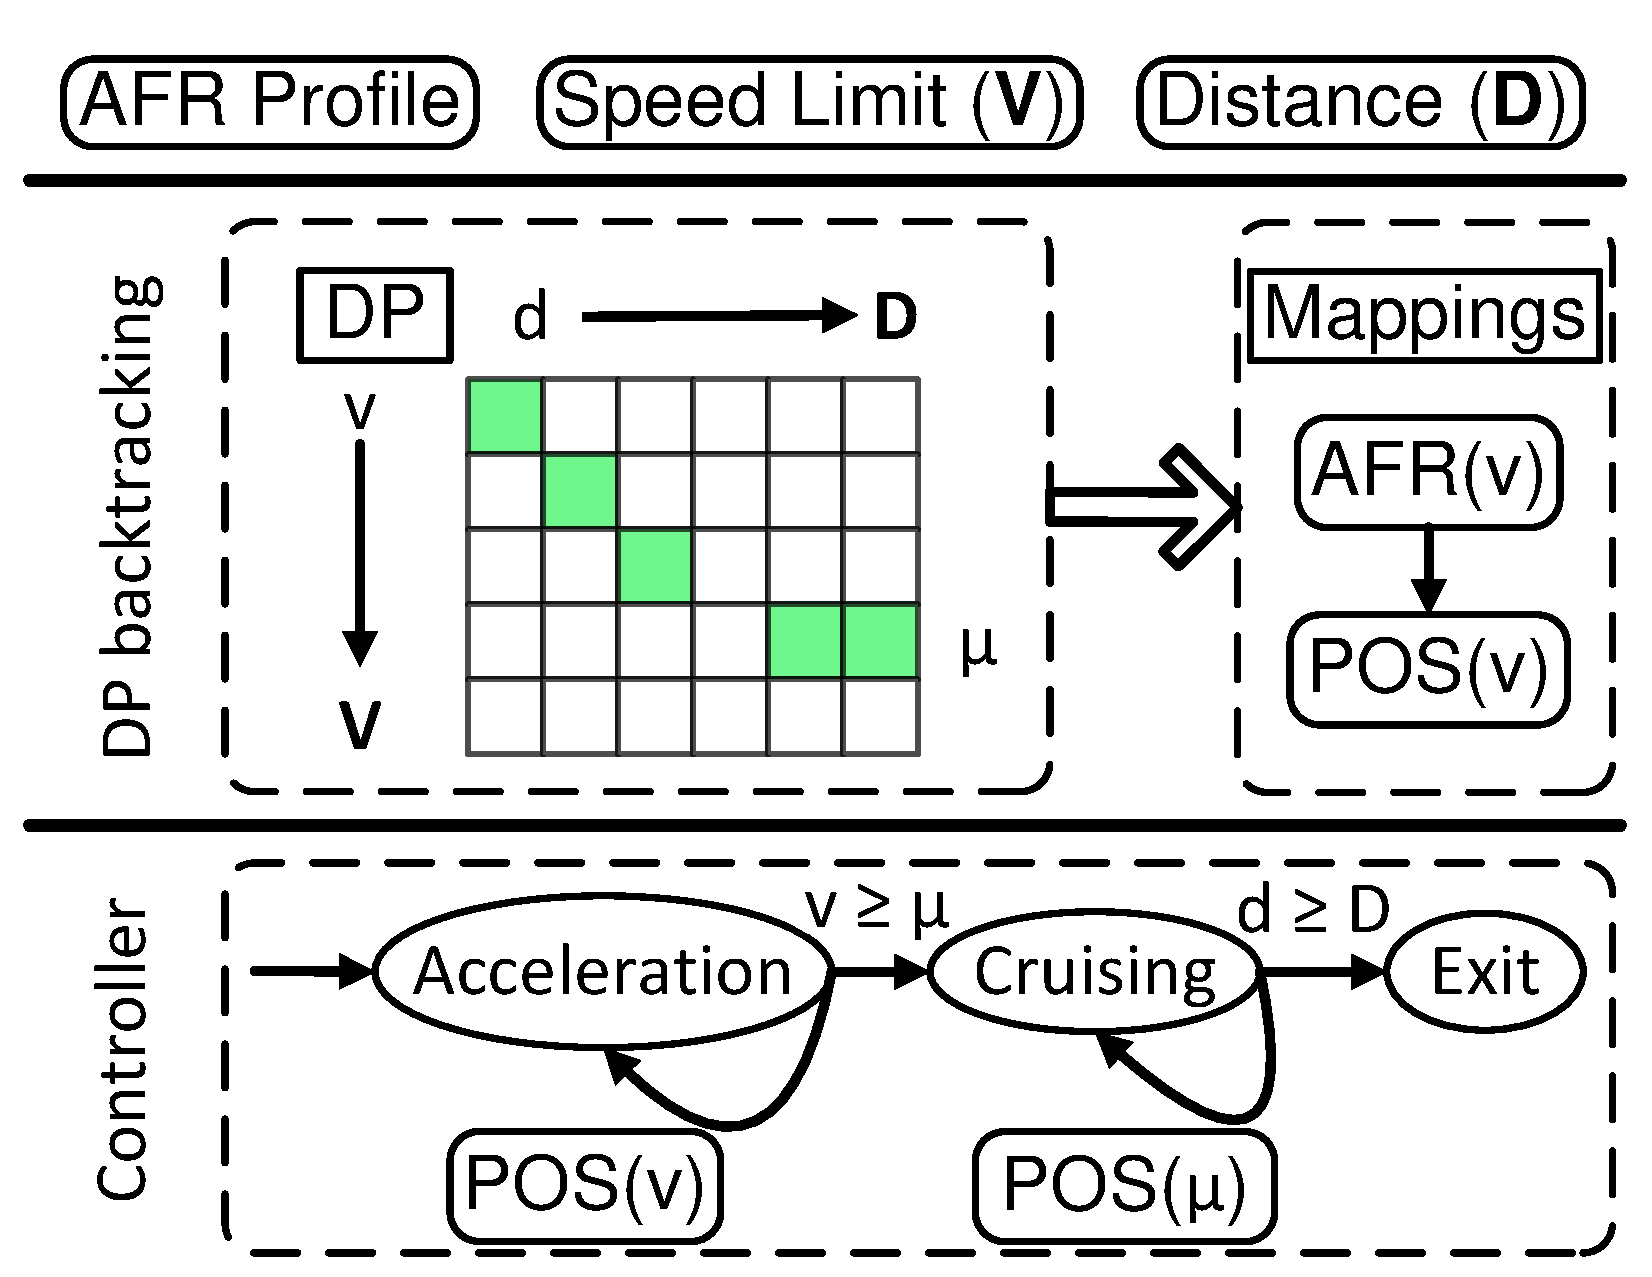
\includegraphics[width=4.0in,angle=0]{Figs/EcoDrive/controlflow.pdf}
\vspace{-0.0cm}
\caption{EcoDrive control flow.}
\vspace{-0.5cm}
\label{controlflow}
\end{center}
\end{figure}



We summarize the control flow of EcoDrive in Fig. \ref{controlflow}. 
The AFR profile is calculated offline by the modeling component. 
Given the travel distance $D$ and speed limit $V$, 
EcoDrive uses dynamic programming model to calculate the speed
to acceleration mapping of the most economic driving strategy. 
This process is done by backtracking the last state of target speed $\mu$. 
The speed to acceleration mapping records the desired
acceleration under that speed. 
This mapping is converted into speed to air/fuel injection rate
mapping $AFR(v)$ by querying the AFR profile. 
The acceleration controller retrieves the air/fuel injection
rate based on the mapping and real-time sensed vehicular speed. 
A air/fuel rate to gas pedal position mapping and 
a gas pedal position to voltage mapping are calculated in advance.
The controller gets the speed to gas pedal position mapping $POS(v)$.  
Based on the air/fuel injection rate, EcoDrive sends 
corresponding voltage values to the ECU. 
In this process, EcoDrive maintains three states, 
acceleration, cruising and exit. 
EcoDrive is in acceleration state by default and enters
cruising state when sensed OBD speed is not less than target speed. 
After it enters cruising state, it remains constant air/fuel
rate injection. 
Different from traditional cruising control, 
EcoDrive may increase/decrease speed in cruising state
by adapting to various road conditions. 
If the car reaches the distance or EcoDrive is turned off
by switch of brake, it enters exit state. 
EcoDrive releases all the resources in exit state
and aborts to wait for next inputs. 


